
\documentclass{beamer}

\usepackage{mathtools}
\usepackage{graphicx}

\usetheme{Pittsburgh}
\usecolortheme{lily}

\definecolor{cwcgray}{rgb}{0.373,0.373,0.373}
\definecolor{cwcblack}{rgb}{0.2,0.2,0.2}

\graphicspath{{../Figures/}}
\DeclareGraphicsExtensions{.eps}

\setbeamercolor{title}{fg=cwcgray}
\setbeamercolor{item}{fg=yellow!50!red}
\setbeamercolor{frametitle}{fg=cwcblack}
\setbeamertemplate{bibliography item}[text]
\setbeamertemplate{background canvas}{\includegraphics[width=\paperwidth]{template}}

\title{\alert{LTE Scheduling Algorithms}}

\author{Ganesh Venkatraman, Tuomo H\"anninen, Antti T\"olli, Le-Nam Tran and Markku Juntti}
\institute{Center for Wireless Communications, DCE, University of Oulu \\ Oulu, Finland 90570}

\date{27.02.2013}

\begin{document}

% Text related command shortcuts

\newcommand{\bi}[1]{\textbf{\textit{#1}}}

% Math related command shortcuts

\newcommand{\mbi}[1]{\mathbf{\mathit{#1}}}
\newcommand{\mbf}[1]{\mathbf{#1}}

\newcommand{\mscrmxy}[2]{{#1}_{\mathrm{#2}}}
\newcommand{\msclxy}[2]{{#1}_{\mathit{#2}}}
\newcommand{\msclxyz}[3]{{#1}_{\mathit{#2},\mathit{#3}}}

\newcommand{\mvecnxy}[2]{\mathbf{#1}_{#2}}
\newcommand{\mvecnxyz}[3]{\mathbf{#1}_{#2,#3}}
\newcommand{\mvecxy}[2]{\mathbf{#1}_{\mathit{#2}}}
\newcommand{\mvecxyz}[3]{\mathbf{#1}_{\mathit{#2},\mathit{#3}}}

\newcommand{\me}[1]{\(#1\)}
\newcommand{\mrm}[1]{\mathrm{#1}}
\newcommand{\mc}[1]{\mathcal{#1}}
\newcommand{\mtext}[1]{\mathit{#1}}

\newcommand{\mxu}[2]{\mathbf{#1}^{\mathit{#2}}}
\newcommand{\mxl}[2]{\mathbf{#1}_{\mathit{#2}}}
\newcommand{\mxul}[3]{\mathbf{#1}^{\mathit{#2}}_{\mathit{#3}}}

\newcommand{\inm}{\, \in \,}
\newcommand{\fall}{\, \forall \,}
\newcommand{\bs}{\: \backslash \:}
\newcommand{\card}[1]{| \, #1 \, |}
\newcommand{\norm}[2]{\|\, #1 \,\|_{#2}}
\newcommand{\gnorm}[1]{\|\, #1 \,\|}
\newcommand{\sset}{\, \subset \,}

\newcommand{\inmt}[1]{\( \mathit{#1} \)}
\newcommand{\mcxy}[2]{\mathcal{#1}_{\mathit{#2}}}

\newcommand{\matbcont}[1]{\left ( \, #1 \, \right )}
\newcommand{\matscont}[1]{\left [ \, #1 \, \right ]}
\newcommand{\setcont}[1]{\lbrace \, #1 \, \rbrace}

\newcommand{\argmax}{\operatorname*{\arg\,max}}

% Math environment command shortcuts

\newenvironment{ceq}{\begin{center}\begin{equation}}{\end{equation}\end{center}}
\newenvironment{cneq}{\begin{center}\begin{equation*}}{\end{equation*}\end{center}}

\newenvironment{ceqn}{\begin{center}\begin{eqnarray}}{\end{eqnarray}\end{center}}
\newenvironment{cneqn}{\begin{center}\begin{eqnarray*}}{\end{eqnarray*}\end{center}}


\begin{frame}
\titlepage
\end{frame}

\begin{frame}
\frametitle{Outline}
\tableofcontents
\end{frame}

\section{Motivation}

\begin{frame}{Introduction and Motivation}
\begin{itemize}
  \item MU-MIMO transmission provides improved data rate
  \item Upcoming standards are moving towards multi-antenna transmission
  \item Multiplexing users spatially provides additional throughput enhancement
  \item Multiplexing of users spatially requires proper selection of user channels to provide interference free transmission
  \item Multi user diversity provides significant improvement over conventional SU-MIMO
  \item User selection for certain objective requires knowledge about user related variables for efficient utilization of the available spectrum
\end{itemize}
\end{frame}

\begin{frame}
\frametitle{}
\begin{block}{Notations}
\begin{itemize}
  \item \me{N_\mrm{T}} - number of transmit antenna
  \item \me{N_\mrm{B}} - number of BS's in the system
  \item \me{K} - number of users in the system
  \item \me{\mc{B}} - set of BS's in the system
  \item \me{\mc{U}} - set of users in the system
  \item \me{\mc{U}_b} - set of users linked to BS \me{b}
  \item \me{\mc{S}_b} - transmission user set
  \item \me{\mvecxyz{h}{b}{k}} - channel between BS \me{b} to user \me{k}
\end{itemize}
\end{block}
\begin{block}{Assumptions}
\begin{itemize}
  \item ZF / WMMSE based precoder design is used for MU-MIMO transmission \cite{wiesel2008zero,wmmse_shi}
  \item \me{\lambda} arrival rate is modeled as Poisson process
\end{itemize}
\end{block}
\end{frame}

\section{Existing Algorithms}

\begin{frame}
\frametitle{Literature Survey}
\begin{block}{SISO Scheduling}
\begin{itemize}
  \item Round Robin Scheduling
  \item Greedy Scheduling
  \item Proportional Fair Scheduling
\end{itemize}
\end{block}
\begin{block}{MU-MIMO Scheduling}
\begin{itemize}
  \item Successive Projection Scheduling \cite{sus2006zfbf}
  \begin{eqnarray*}
  \mbf{N} &=& \mbf{I} - \mbf{U} ( \, \mbf{U}^\mrm{H} \mbf{U} \, )^{-1} \mbf{U}^\mrm{H} \\
  \mbf{U} &=& \matscont{\mvecxyz{h}{b}{x}^\mrm{T} \; \mvecxyz{h}{b}{y}^\mrm{T}} \fall x,y \inm \mc{S}_b \text{ where } b \inm \mc{B}
  \end{eqnarray*}
  \item selection is based on the following
  \begin{equation}
  j = \argmax_i \gnorm{\mbf{N}^\mrm{H} \mvecxyz{h}{b}{i}^\mrm{T}} \, \fall i \inm \mc{U}_b \nonumber
  \end{equation}

\end{itemize}
\end{block}
\end{frame}

\section{Single BS Selection}

\subsection{Sum Capacity maximization}

\begin{frame}
\begin{block}{Pair-Wise User Selection}
\begin{itemize}
  \item Selection is based on pair-wise user metric
  \item Diagonal entries are populated with the channel norms
  \begin{eqnarray*}
  \mbf{T} &=& \left [\,\mbf{T}_\mrm{o} \; \mvecxy{h}{i}^\mrm{T} \, \right ] \\
  \msclxyz{M}{i}{i} &=& \det{\left ( \, \mbf{T}^{\mrm{H}} \; \mbf{T} \, \right )}
  \end{eqnarray*}
  \item Non diagonal entries are filled with the volume subtended between two user channel vectors
  \begin{eqnarray*}
  \mbf{T} &=& \left [\,\mbf{T}_\mrm{o} \; \mvecxy{h}{i}^\mrm{T} \; \mvecxy{h}{j}^\mrm{T} \, \right ] \\
  \msclxyz{M}{i}{j} &=& \det{\left ( \, \mbf{T}^{\mrm{H}} \; \mbf{T} \, \right )}
  \end{eqnarray*}
  \item EVD with \me{\mvecxy{p}{i}} where \me{i = \argmax_k \msclxyz{D}{k}{k}} where \me{\mbf{M} = \mbf{P} \mbf{D} \mbf{P}^\mrm{H}} \cite{saaty2008decision}
  \begin{eqnarray*}
  i &=& \argmax_{\mathrm{i}} \norm{\msclxyz{p}{i}{k}}{2} \\
  \mc{S} &=& \left \lbrace \, \mc{S} \, \cup \, i \, \right \rbrace.
  \end{eqnarray*}
\end{itemize}
\end{block}
\end{frame}

\begin{frame}
\begin{block}{Reduced Null Space based User Selection}
\begin{itemize}
  \item Selection is based on successive projections discussed earlier
  \item Null space is approximated by the product of perpendiculars
  \begin{eqnarray*}
  \mbf{U} = \left [ \, \frac{\mvecxy{h}{i}^\mrm{T}}{\gnorm{\mvecxy{h}{i}}}, \dotsc, \frac{\mvecxy{h}{j}^\mrm{T}}{\gnorm{\mvecxy{h}{j}}} \, \right ], \; \fall i,j \inm \mc{S}
  \end{eqnarray*}
  \item Vertical distance is calculated by the following metric
  \begin{equation*}
  \mbf{g} = \mbf{U}^\mrm{H} \mvecxy{h}{i}^\mrm{T}, \fall i \inm \mc{U}
  \end{equation*}
  \item Null space is approximated by the following
  \begin{equation*}
  \msclxy{m}{i} = \prod^{\card{\mc{S}}}_{l = 1} \left ( \, \gnorm{\mvecxy{h}{i}} - \card{g_l} \, \right ), \fall i \inm \mc{U}
  \end{equation*}
  \item Selection is as discussed earlier
\end{itemize}
\end{block}
\end{frame}

\subsection{Queue Minimizing Algorithms}

\begin{frame}
\begin{block}{Queue Weighted Successive Projections}
\begin{itemize}
  \item Selection is based on minimizing the expected queue backlogs of all users
  \item Lyapunov drift \cite{neely2010stochastic} for single user is extended for MU-MIMO scenario as
  \begin{eqnarray*}
  &\displaystyle \max_{\mc{S} \inm \mc{U}} \, \sum_{i \inm \mc{S}}\mbf{Q}_i(n) \, \mbf{b}_i(n) \\
  &\displaystyle \mrm{subject \: to,} \quad \card{\mc{S}} \leq N_\mrm{T}
  \end{eqnarray*}
  \item With the following formulation
  \begin{eqnarray*}
  &\displaystyle \max_{\fall i \inm \mc{U}} \, \mbf{Q}_i \, \log \left \lbrace 1 + \frac{P_\mrm{i} \; \gnorm{\mvecxy{h}{i}}^2}{N_\mrm{0}} \right \rbrace \\
  &\displaystyle \max_{\fall i \inm \mc{U}} \, \mbf{Q}_i \, \left [ \; 2 \, \log \left \lbrace P_\mrm{i} \; \gnorm{\mvecxy{h}{i}} \right \rbrace - \log \left \lbrace N_\mrm{0} \right \rbrace \; \right ]
  \end{eqnarray*}
  \item Approximate solution is given by \me{\max_i \mbf{Q}_i \: \mvecxy{h}{i}} where \me{\log \{x \} \approx x}
\end{itemize}
\end{block}
\end{frame}

\begin{frame}
\begin{block}{Percentile Proportional Fairness}
\begin{itemize}
  \item Successive projection based user search is performed
  \item Reduced user set is based on PF metric which is given by \me{f_i = {\mbf{r}_i \mbf{Q}_i} / {\mbf{R}_i}}
  \item Reduced user set \me{\mc{S}_\pi} is then grouped by
  \begin{equation*}
  \mc{S}_\pi = \left \lbrace \: i \mid \arg_i \: \msclxyz{f}{\pi}{i} \geq \msclxyz{f}{\pi}{x}, \fall i \inm \mc{U} \: \right \rbrace
  \end{equation*}
  where \me{x = 50} corresponds to \me{50 \% \: \text{ile}} user selection.
  \item Selection over this set is then performed by successive projection discussed earlier with queue weighted projections
  \item Users in \me{\mc{S}^c_\pi = \mc{U} \bs \mc{S}_\pi} are having lower PF metric which provides better fairness
  \item Selection has lower complexity while achieving significant fairness and sum capacity
\end{itemize}
\end{block}
\end{frame}

\subsection{Plots}

\begin{frame}
\begin{figure}
\centering
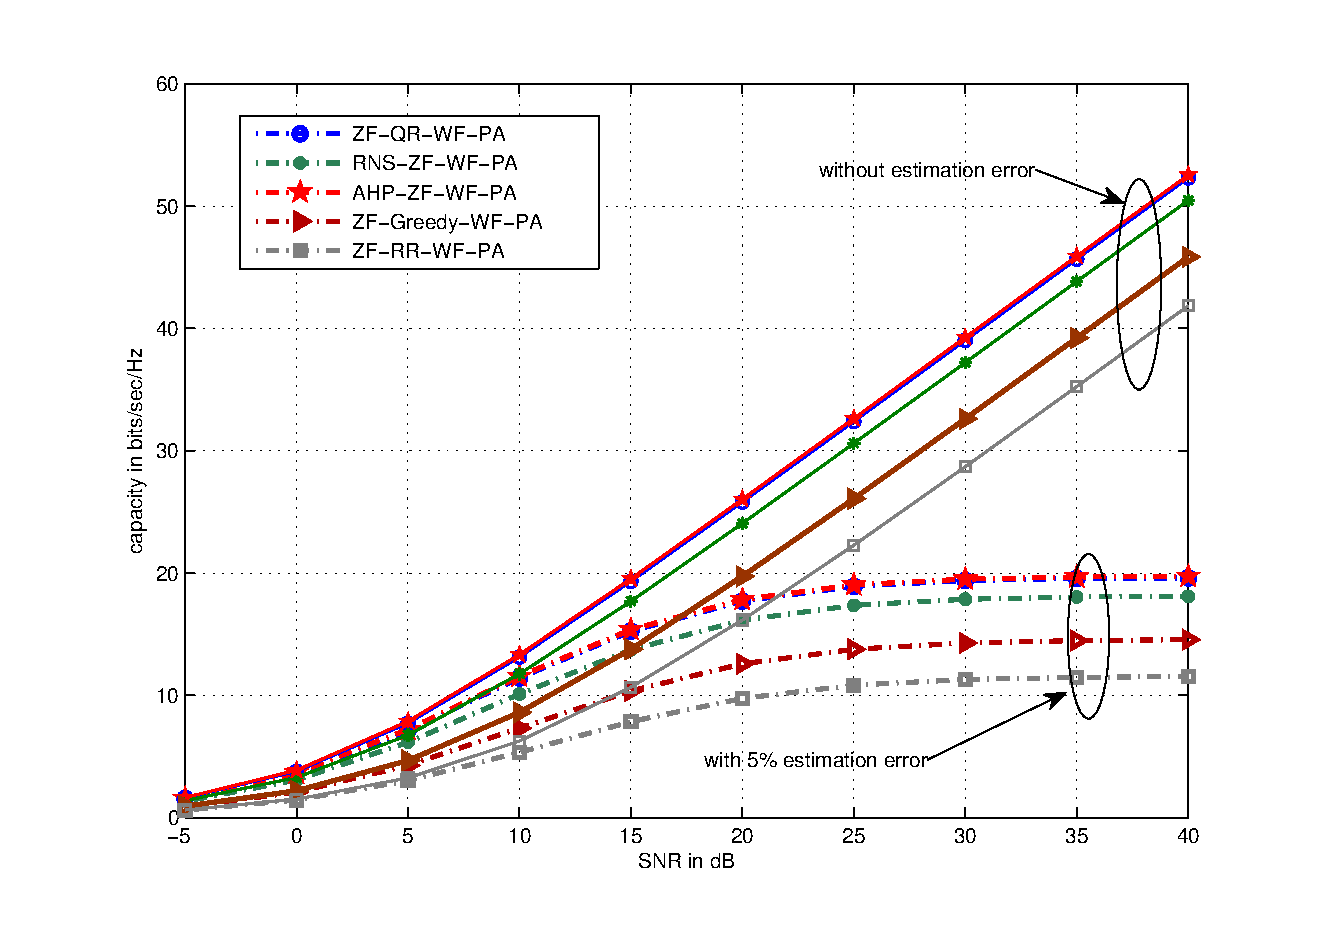
\includegraphics[width=0.8\textwidth]{single-bs-1}
\caption[short]{Sum capacity for \me{\card{\mc{U}} = 20, \, N_\mrm{T} = 4, \, N_\mrm{R} = 1}}
\label{single-bs-f1}
\end{figure}
\end{frame}

\begin{frame}
\begin{figure}
\centering
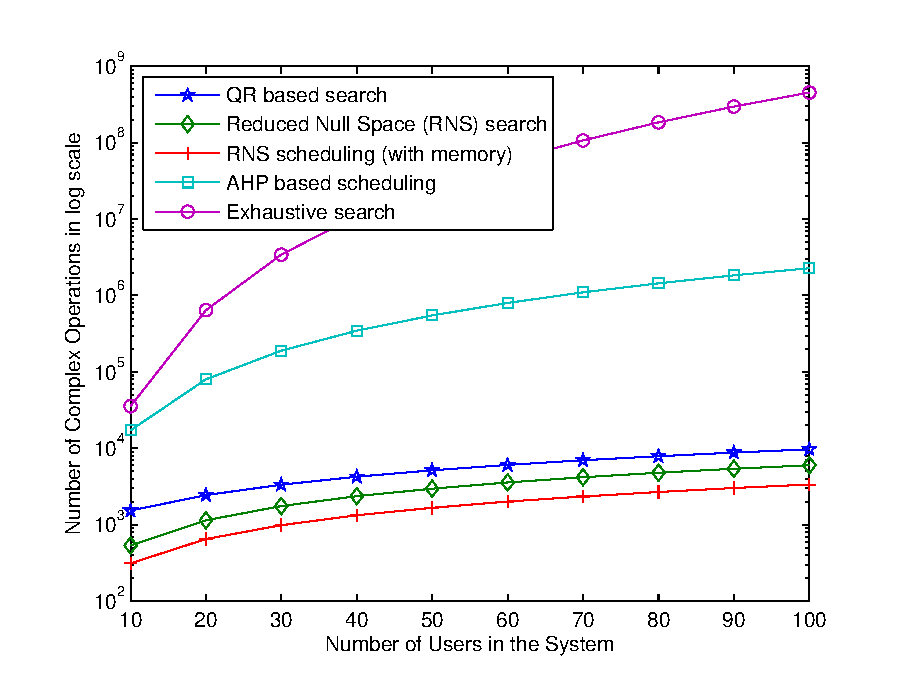
\includegraphics[width=0.8\textwidth]{single-bs-2}
\caption[short]{Scaling of complexity over users for \me{N_\mrm{T} = 4, \, N_\mrm{R} = 1} system}
\label{single-bs-f2}
\end{figure}
\end{frame}

\begin{frame}
\begin{figure}
\centering
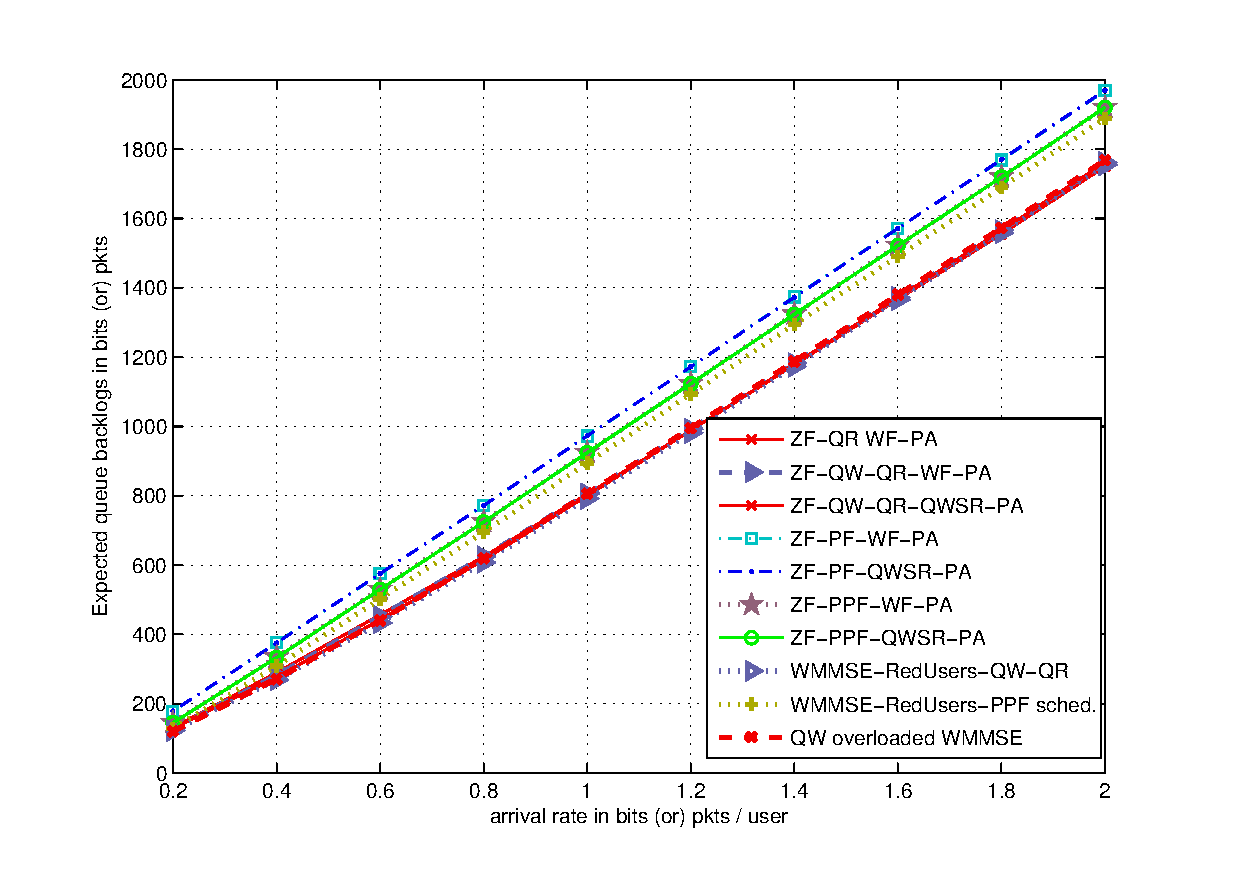
\includegraphics[width=0.8\textwidth]{single-bs-3}
\caption[short]{Expected queue size \me{\card{\mc{U}} = 50, \, N_\mrm{T} = 4, \, N_\mrm{R} = 1, \, \mc{U}(0,-30)} over \me{1000} slots at \me{15}dB SNR}
\label{single-bs-f3}
\end{figure}
\end{frame}

\begin{frame}
\begin{figure}
\centering
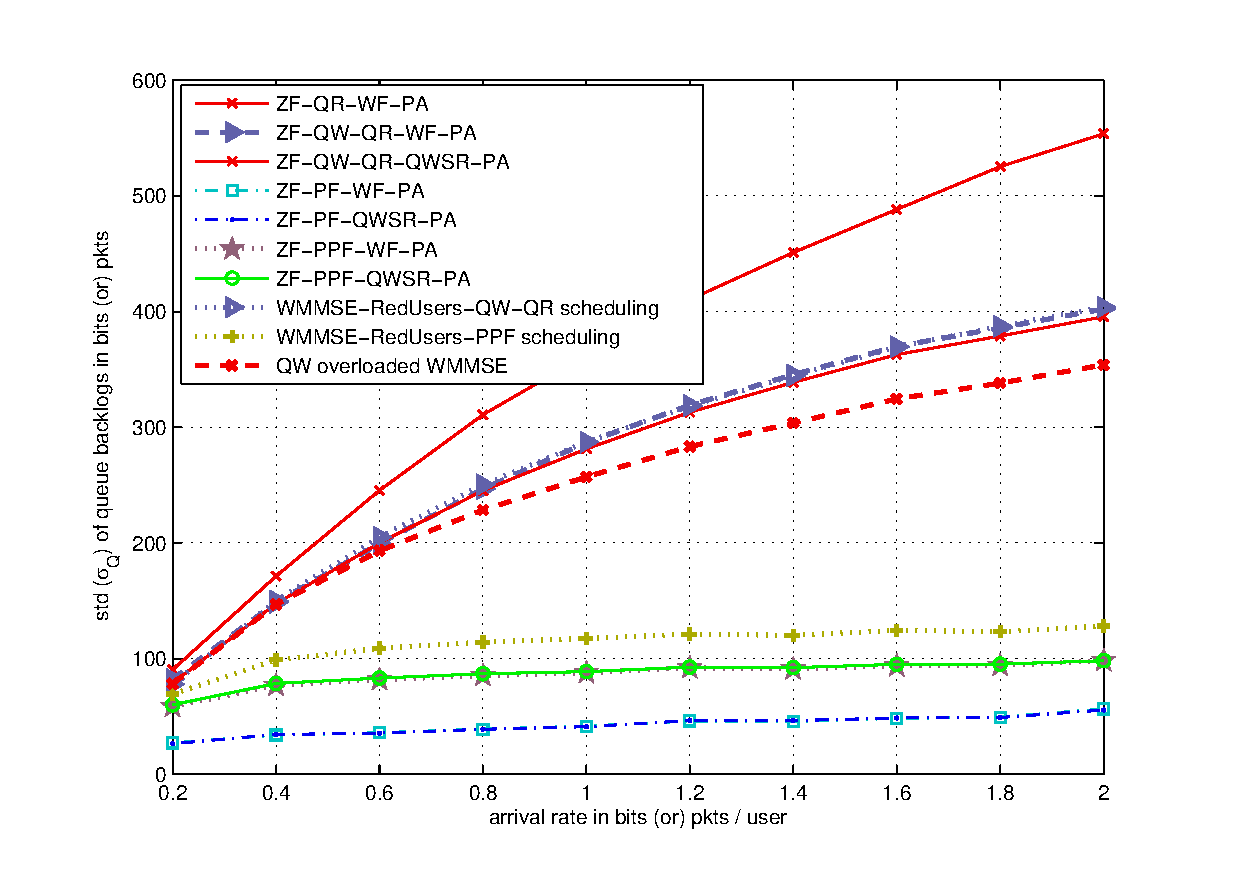
\includegraphics[width=0.8\textwidth]{single-bs-4}
\caption[short]{Standard deviation of backlogged packets \me{\card{\mc{U}} = 50, \, N_\mrm{T} = 4, \, N_\mrm{R} = 1, \, \mc{U}(0,-30)} over \me{1000} slots at \me{15}dB SNR}
\label{single-bs-f4}
\end{figure}
\end{frame}

\section{Multi BS Scheduling}

\subsection{Static User Selection}

\begin{frame}
\begin{block}{Static User Scheduling}
\begin{itemize}
  \item Each BS selects \me{\left \lfloor \frac{N_\mrm{T}}{N_\mrm{B}} \right \rfloor} with the assumption \me{N_\mrm{T} \geq N_\mrm{B}}
  \item Users are selection in an iterative manner by updating each BS with the set \me{\mc{S}_b} for each BS \me{b}
  \item Each BS select users based on the following metric
  \begin{equation*}
  \begin{array}{lcl}
  d_k &=& \det \matbcont{\mbf{T}^\mrm{H} \; \mbf{T}} \\
  \mbf{T} &=& \matscont{\mbf{T}_\mrm{X} \; \mbf{T}_\mrm{D} \; \mvecxyz{h}{j}{i}^\mrm{T}}, \fall i \inm \mc{U}_j
  \end{array}
  \end{equation*}
  \item where \me{\mbf{T}_{\mrm{D}} \, \mtext{and} \, \mbf{T}_{\mrm{X}}} are given by
  \begin{equation*}
  \begin{array}{lcl}
  \mbf{T}_{\mrm{D}} &=& \matscont{\mvecxyz{h}{j}{k}^\mrm{T} \dotso}, \fall k \inm \mc{S}_j \\
  \mbf{T}_{\mrm{X}} &=& \matscont{\mvecxyz{h}{j}{k}^\mrm{T} \dotso }, \fall k \inm \displaystyle \bigcup_{\mathclap{\fall b \inm \mc{B} \bs j}} \mc{S}_b.
  \end{array}
  \end{equation*}
  \item BS will select the user independently after the update as given by \me{\hat{k} = \argmax_k \, d_k} as \me{\mc{S}_j = \setcont{\mc{S}_j \cup \hat{k}}}
\end{itemize}
\end{block}
\end{frame}

\subsection{Coordinate User Selection}

\begin{frame}
\begin{block}{Coordinate User Scheduling}
\begin{itemize}
  \item User can be associated with any BS at a given instant
  \item Initial user is selected as \me{ \mc{S}_{\hat{b}} = \setcont{\mc{S}_{\hat{b}} \cup \hat{k}}}
  \item Metric used is given by \me{\{\, \hat{b},\hat{k} \,\} \: = \: \argmax_{b,k} \gnorm{\mvecxyz{h}{b}{k}}}
  \item Each BS will then perform the following metric to select the user
  \begin{equation*}
  \begin{array}{lcl}
  D_{j,i} &=& \det \left ( \; \mbf{T}^{\mrm{H}} \; \mbf{T} \; \right ) \\
  \mbf{T} &=& \matscont{\mbf{T}_\mrm{X} \; \mbf{T}_\mrm{D} \; \mvecxyz{h}{j}{i}^\mrm{T}}, \fall i \inm \mc{U}
  \end{array}
  \end{equation*}
  \item Inter and Intra cell components for each BS is updated as
  \begin{equation*}
  \begin{array}{lcl}
  \mbf{T}_{\mrm{D}} &=& \matscont{\mvecxyz{h}{j}{k}^\mrm{T} \dotso}, \fall k \inm \mc{S}_j \\
  \mbf{T}_{\mrm{X}} &=& \matscont{\mvecxyz{h}{j}{k}^\mrm{T} \dotso }, \fall k \inm \displaystyle \bigcup_{\mathclap{\fall b \inm \mc{B} \bs j}} \mc{S}_b
  \end{array}
  \end{equation*}
  \item The BS and the corresponding user is identified by \me{ \{ \, \hat{b},\hat{k} \,\} = \argmax_{i,j} \quad D_{i,j} \; \fall i \inm \mc{U} \text{ and } \fall j \inm \mc{B} }
\end{itemize}
\end{block}
\end{frame}

\subsection{Plots}

\begin{frame}
\begin{figure}
\centering
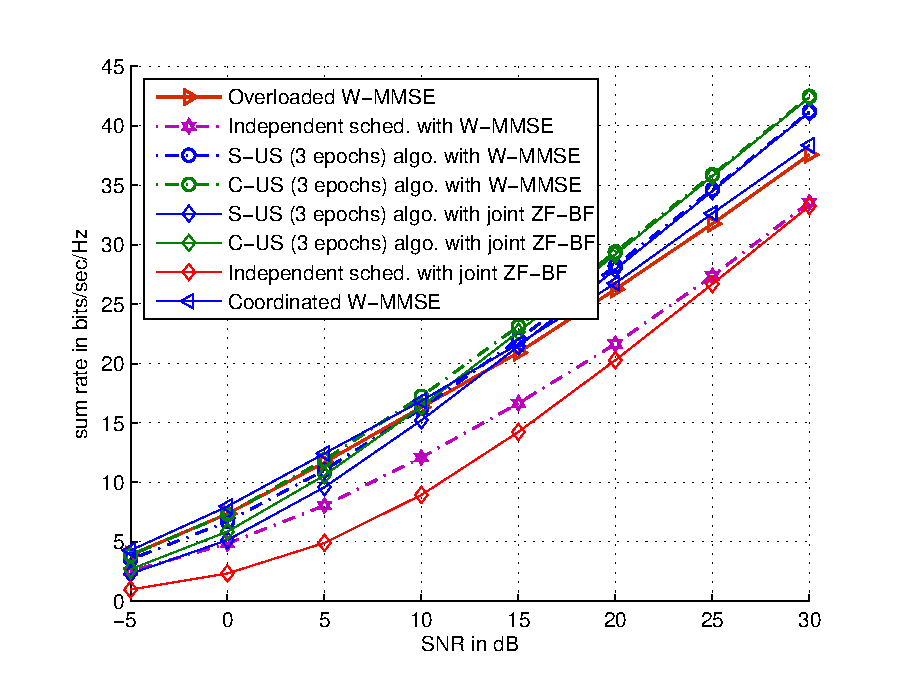
\includegraphics[width=0.8\textwidth]{multi-bs-1}
\caption[short]{Sum capacity for \me{\card{\mc{B}} = 2, \, \card{\mc{U}_k} = 25, \, N_\mrm{T} = 4, \, N_\mrm{R} = 1}}
\label{multi-bs-f1}
\end{figure}
\end{frame}

\begin{frame}
\begin{figure}
\centering
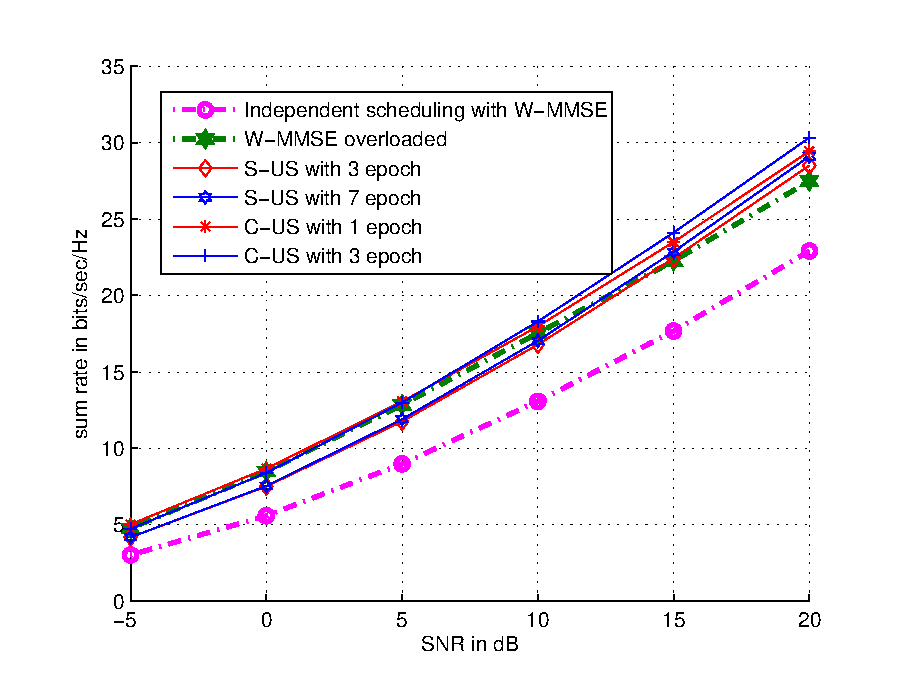
\includegraphics[width=0.8\textwidth]{multi-bs-2}
\caption[short]{Iterative sum capacity for \me{\card{\mc{B}} = 2, \, \card{\mc{U}} = 20, \, N_\mrm{T} = 4, \, N_\mrm{R} = 1}}
\label{multi-bs-f2}
\end{figure}
\end{frame}

\begin{frame}{Conclusion}
\begin{itemize}
  \item We analyzed the selection strategies with the objective of queue size reduction and capacity maximization
  \item Complexity involved with the selection process is also addressed
  \item Multi BS user selection provides significantly better performance by iterating it over the BSs
  \item Coordinate scheduling provides improved performance over Static user scheduling when users are at the cell-edge
  \item Delay constrained user scheduling should be considered in the future work
\end{itemize}
\end{frame}

\begin{frame}{Bibligraphy}
\scriptsize {\bibliographystyle{ieeetr}
\bibliography{./../Library/kirja_survey}}
\end{frame}

\end{document}
